\chapter{LaTeX-Bausteine}\label{Bausteine}

Der Text wird in bis zu drei Ebenen gegliedert:

\begin{enumerate}
	\item Kapitel (\verb|\chapter{Kapitel}|)\index{Kapitel}
	\item Abschnitte (\verb|\section{Abschnitt}|)
	\item Unterabschnitte (\verb|\subsection{Unterabschnitt}|)
\end{enumerate}

\section{Abschnitt}\index{Abschnitt}

Lorem ipsum dolor sit amet, consetetur sadipscing elitr, sed diam nonumy eirmod tempor invidunt ut labore et dolore magna aliquyam erat, sed diam voluptua \cite{Nannen:03}. At vero eos et accusam et justo duo dolores et ea rebum. Stet clita kasd gubergren, no sea takimata sanctus est Lorem ipsum dolor sit amet. Lorem ipsum dolor sit amet, consetetur sadipscing elitr, sed diam nonumy eirmod tempor invidunt ut labore et dolore magna aliquyam erat, sed diam voluptua. At vero eos et accusam et justo duo dolores et ea rebum. Stet clita kasd gubergren, no sea takimata sanctus est Lorem ipsum dolor sit amet.

\subsection{Unterabschnitt} \index{Unterabschnitt}

Lorem ipsum dolor sit amet, consetetur sadipscing elitr, sed diam nonumy eirmod tempor invidunt ut labore et dolore magna aliquyam erat, sed diam voluptua. At vero eos et accusam et justo duo dolores et ea rebum. Stet clita kasd gubergren, no sea takimata sanctus est Lorem ipsum dolor sit amet. Lorem ipsum dolor sit amet, consetetur sadipscing elitr, sed diam nonumy eirmod tempor invidunt ut labore et dolore magna aliquyam erat, sed diam voluptua. At vero eos et accusam et justo duo dolores et ea rebum. Stet clita kasd gubergren, no sea takimata sanctus est Lorem ipsum dolor sit amet.

\section{Abbildungen und Tabellen}

Abbildung\index{Abbildung} und Tabellen\index{Tabelle} werden zentriert eingefügt. Grundsätzlich sollen sie erst dann erscheinen, nach dem sie im Text angesprochen wurden (siehe Abbildung \ref{a1}). Abbildungen und Tabellen (siehe Tabelle \ref{t1}) können im Fließtext (\verb|h=here|), am Seitenanfang (\verb|t=top|), am Seitenende (\verb|b=bottom|) oder auch gesammelt auf einer nachfolgenden Seite (\verb|p=page|) oder auch ganz am Ende der Ausarbeitung erscheinen. Letzteres sollte man nur dann wählen, wenn die Bilder günstig zusammen zu betrachten sind und die Ausarbeitung nicht zu lang ($< 20$ Seiten) ist.

\begin{figure} %[hbtp]
	\centering
	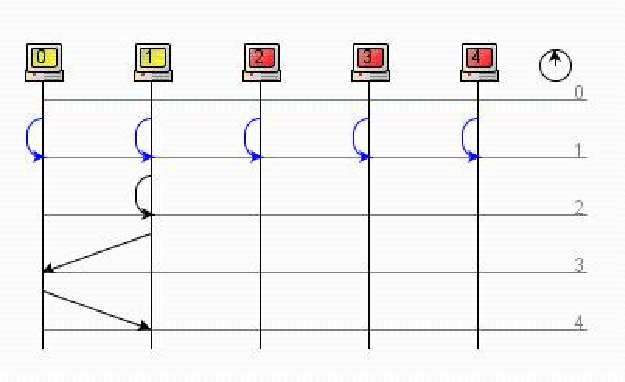
\includegraphics{images/sequence.pdf}
	\caption{Bezeichnung der Abbildung}
	\label{a1}
\end{figure}

\begin{table} %[hbtp]
	\centering
	\begin{tabular}{l | l l l l}
		\textbf{Prozesse} & \textbf{Zeit} $\rightarrow$ \\
		\hline
		$P_{1}$ & $W(x)1$ \\
		$P_{2}$ & & $W(x)2$ \\
		$P_{3}$ & & $R(x)2$ & & $R(x)1$\\
		$P_{4}$ & & & $R(x)2$ & $R(x)1$\\
	\end{tabular}
	\caption{Bezeichnung der Tabelle}
	\label{t1}
\end{table}

\section{Listings}\index{Quelltext}\index{Listing}

Lorem ipsum dolor sit amet, consetetur sadipscing elitr, sed diam nonumy eirmod tempor invidunt ut labore et dolore magna aliquyam erat, sed diam voluptua (siehe Listing \ref{quicksort.py}, Zeile 8).

\begin{lstlisting}[language=Python, caption={Quicksort-Implementierung in Python}\label{quicksort.py}]
def quicksort(arr):
less = []
pivotList = []
more = []
if len(arr) <= 1:
	return arr
else:
	pivot = arr[0]	# the pivot element
	for i in arr:
		if i < pivot:
			less.append(i)
		elif i > pivot:
			more.append(i)
		else:
			pivotList.append(i)
	less = quicksort(less)
	more = quicksort(more)
	return less + pivotList + more

print(quicksort[4, 65, 2, -31, 0, 99, 83, 782, 1]))
\end{lstlisting}

Lorem ipsum dolor sit amet, consetetur sadipscing elitr, sed diam nonumy eirmod tempor invidunt ut labore et dolore magna aliquyam erat, sed diam voluptua (siehe Listing \ref{quicksort.js}, Zeilen 3 und 5).

\begin{lstlisting}[caption={Quicksort-Implementierung in JavaScript}\label{quicksort.js}]
function quicksort([pivot, ...others]) {
	return pivot === undefined ? [] : [
		...quicksort(others.filter(n => n < pivot)),
		pivot,
		...quicksort(others.filter(n => n >= pivot))
	];
}

console.log(quicksort([11.8, 14.1, 21.3, 8.5, 16.7, 5.7]));
\end{lstlisting}

Größere Code-Fragmente sollten im Anhang eingefügt werden. \cite{wiki:listing}

\section{Mathematische Formel}\index{Formel}

Mathematische Formeln bzw. Formulierungen können sowohl im Fließtext (z.B. $y=x^2$) oder abgesetzt und zentriert im Text erscheinen. Gleichungen sollten für Referenzierungen nummeriert werden (siehe Formel \ref{gl-1}).

\begin{equation}
	\label{gl-1}
	e_{i}=\sum _{i=1}^{n}w_{i}x_{i}
\end{equation}

Entscheidungsformel:

\begin{equation}
	\psi(t)=\left\{\begin{array}{ccc}
		1 & \qquad 0 <= t < \frac{1}{2} \\
		-1 & \qquad \frac{1}{2} <= t <1 \\
		0 & \qquad sonst
	\end{array} \right.
\end{equation}

Matrix:\index{Matrix}

\begin{equation}
A = \left(
	\begin{array}{llll}
		a_{11} & a_{12} & \ldots & a_{1n} \\
		a_{21} & a_{22} & \ldots & a_{2n} \\
		\vdots & \vdots & \ddots & \vdots \\
		a_{n1} & a_{n2} & \ldots & a_{nn} \\
	\end{array}
\right)
\end{equation}

Vektor:\index{Vektor}

\begin{equation}
	\overline{a} = \left(
		\begin{array}{c}
			a_{1}\\
			a_{2}\\
			\vdots\\
			a_{n}\\
		\end{array}
	\right)
\end{equation}

\section{Sätze, Lemmata, Definitionen, Beweise, Beispiele}\index{Satz}\index{Lemma}\index{Definition}\index{Beweis}\index{Beispiel}

Sätze, Lemmata, Definitionen, Beweise und Beispiele können in speziell dafür vorgesehenen Umgebungen erstellt werden.

\begin{definition}(Optimierungsproblem)
Ein \emph{Optimierungsproblem} $\mathcal{P}$ ist festgelegt durch ein Tupel $(I_\mathcal{P}, sol_\mathcal{P}, m_\mathcal{P}, goal)$ wobei gilt

\begin{enumerate}
	\item $I_\mathcal{P}$ ist die Menge der Instanzen,
	\item $sol_\mathcal{P} : I_\mathcal{P} \longmapsto \mathbb{P}(S_\mathcal{P})$ ist eine Funktion, die jeder Instanz $x \in I_\mathcal{P}$ eine Menge zulässiger Lösungen zuweist,
	\item $m_\mathcal{P} : I_\mathcal{P} \times S_\mathcal{P} \longmapsto \mathbb{N}$ ist eine Funktion, die jedem Paar $(x,y(x))$ mit $x \in I_\mathcal{P}$ und $y(x) \in sol_\mathcal{P}(x)$ eine Zahl $m_\mathcal{P}(x,y(x)) \in \mathbb{N}$ zuordnet (= Maß für die Lösung $y(x)$ der Instanz $x$), und
	\item $goal \in \{min,max\}$.
\end{enumerate}
\end{definition}

\begin{example}
	MINIMUM TRAVELING SALESMAN (MIN-TSP)
	\begin{itemize}
		\item $I_{MIN-TSP} =_{def}$ s.o., ebenso $S_{MIN-TSP}$
		\item $sol_{MIN-TSP}(m,D) =_{def} S_{MIN-TSP} \cap \mathbb{N}^m$
		\item $m_{MIN-TSP}((m,D),(c_1, \ldots , c_m)) =_{def} \sum_{i=1}^{m-1} D(c_i, c_{i+1}) + D(c_m,c_1)$
		\item $goal_{MIN-TSP} =_{def} min$
	\end{itemize}
	\begin{flushright}$\qed$\end{flushright}
\end{example}

\begin{theorem}
Sei $\mathcal{P}$ ein \textbf{NP}-hartes Optimierungsproblem. Wenn $\mathcal{P} \in$ \textbf{PO}, dann ist \textbf{P} = \textbf{NP}.
\end{theorem}

\begin{proof}
Um zu zeigen, dass \textbf{P} = \textbf{NP} gilt, genügt es wegen Satz A.30 zu zeigen, dass ein einziges \textbf{NP}-vollständiges Problem in \textbf{P} liegt. Sei also $\mathcal{P}'$ ein beliebiges \textbf{NP}-vollständiges Problem.

Weil $\mathcal{P}$ nach Voraussetzung \textbf{NP}-hart ist, gilt insbesondere $\mathcal{P}' \leq_T \mathcal{P}_C$. Sei $R$ der zugehörige Polynomialzeit-Algorithmus dieser Turing-Reduktion. Weiter ist $\mathcal{P} \in$ \textbf{PO} vorausgesetzt, etwa vermöge eines Polynomialzeit-Algorithmus $A$. Aus den beiden Polynomialzeit-Algorithmen $R$ und $A$ erhält man nun leicht einen effizienten Algorithmus für $\mathcal{P}'$: Ersetzt man in $R$ das Orakel durch $A$, ergibt dies insgesamt eine polynomielle Laufzeit.

%\begin{flushright}$\qed$% \end{flushright}
\end{proof}

\begin{lemma}
Aus \textbf{PO} $=$ \textbf{NPO} folgt \textbf{P} $=$ \textbf{NP}.
\end{lemma}

\begin{proof}
Es genügt zu zeigen, dass unter der angegeben Voraussetzung KNAPSACK $\in$ \textbf{P} ist.

Nach Voraussetung ist MAXIMUM KNAPSACK $\in$ \textbf{PO}, d.h. die Berechnung von $m^*(x)$ für jede Instanz $x$ ist in Polynomialzeit möglich. Um KNAPSACK bei Eingabe $(x,k)$ zu entscheiden, müssen wir nur noch $m^*(x) \geq k$ prüfen. Ist das der Fall, geben wir $1$, sonst $0$ aus. Dies bleibt insgesamt ein Polynomialzeit-Algorithmus.

\begin{flushright}$\qed$\end{flushright}
\end{proof}

\section{Fußnoten}

In einer Fußnote können ergänzende Informationen\footnote{Informationen die für die Arbeit zweitrangig sind, jedoch für den Leser interessant sein könnten.} angegeben werden. Außerdem kann eine Fußnote auch Links enthalten. Wird in der Arbeit eine Software (zum Beispiel Java\footnote{\url{https://www.oracle.com/java/technologies/}}) eingesetzt, so kann die Quelle, die diese Software zur Verfügung stellt in der Fußnote angegeben werden.

\section{Literaturverweise}\index{Literatur}\index{Quellen}

Alle benutzte Literatur wird im Literaturverzeichnis angegeben\footnote{Dazu wird eine sogenannte BibTeX-Datei (literatur.bib) verwendet.}. Alle angegebene Literatur sollte mindestens einmal im Text referenziert werden \cite{Cormen:90}.
